\clearpage\begingroup\SourceLeaf{73b}\HistoricalHead{68}{L}{PHYSIK. NACHLASS.}
\begin{center}[10.]\end{center}
\noindent{\small [S. 207]}
\begin{center}\textbf{Rotationscommutatoren mit drei Gleisen.}\end{center}
\begin{center}
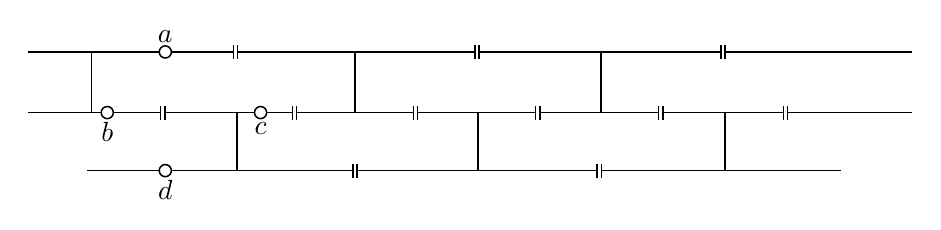
\begin{tikzpicture}[x=.011cm,y=.011cm,line width=.55pt]
\draw (0,140)--(1020,140);
\draw (0,70)--(1020,70);
\draw (68,3)--(938,3);
\draw (73,140)--(73,70) (377,140)--(377,70) (661,140)--(661,70);
\draw (241,70)--(241,3) (519,70)--(519,3) (804,70)--(804,3);
\foreach \x/\y in {158/140,91/70,268/70,158/3}{\draw[fill=white] (\x,\y) circle[radius=7];}
\node[above,inner sep=1pt] at (158,147) {$a$};
\node[below,inner sep=1pt] at (91,63) {$b$};
\node[below,inner sep=1pt] at (268,63) {$c$};
\node[below,inner sep=1pt] at (158,-4) {$d$};
\foreach \x/\y in {239/140,518/140,802/140,155/70,307/70,447/70,588/70,730/70,874/70,377/3,659/3}{
  \draw[white,line width=2pt] (\x,\y-7)--(\x,\y+7);
  \draw (\x-2.4,\y-8)--(\x-2.4,\y+8) (\x+2.4,\y-8)--(\x+2.4,\y+8);
}
\end{tikzpicture}
\end{center}
\indent Die rothen[\textsuperscript{*})] Linien bedeuten metallene Gleise, auf welchen gleichzeitig
die Enden von vier Metalldrähten \(a,b,c,d\) sich bewegen; die schwarzen Einschnitte
sind Unterbrechungen des metallischen Zusammenhanges.
\begingroup\renewcommand{\thefootnote}{}\footnotetext{[\textsuperscript{*}) In der Handschrift sind die Hauptlinien der Zeichnung rot, nur die »Enden« \(a,b,c,d\) und die
hier verdoppelt eingezeichneten »Unterbrechungen« sind schwarz.]}\endgroup
\clearpage\endgroup
